\documentclass[a4paper,12pt]{article}
\usepackage{fullpage}
\usepackage{hyperref}
\usepackage{url}
\usepackage{graphicx}
%\usepackage{polski}
\usepackage[utf8]{inputenc}

\setlength{\parindent}{0pt}
\addtolength{\parskip}{\baselineskip}

\title{3rd Year Group Project\\Report Three\\}

\author{
    \small{Rafał Szymański}\\
  	\and
    \small{Maciek Albin}\\
    \and
    \small{Sam Wong}\\
    \and  
    \small{Suhaib Sarmad}\\
		\and
		\small{Jamal Khan}\\
		\and
		\small{\{rs2909, mja108, sw2309, sss308, jzk09\}@doc.ic.ac.uk}
		\and
		\\Department of Computing - Imperial College London
}

\date{}

\begin{document} 
	\maketitle
	
	\section{Testing}
	
	\section{General Validation}
	
	\section{Managerial Documentation}
	
		\subsection{Collaboration Tools Used}
		
			\subsubsection{Git}
			
			We have used the git version control system for keeping track of the project, for easily reverting if there is a problem, and for having a very quick deploy mechanism. Whenever a code push occurs to our git repository, we have a git post-receive hook that copies the static files appropriately, and restarts the appropriate processes. This means that as soon as a code push occurs, the new version is live.
			
			\subsubsection{Trello}
			
			Trello\footnote{\url{http://trello.com}} is a very good piece of software by FogCreek. It is a digital board that allows you to create post-its and write the product backlog, and move tasks between the product backlog, the current iteration, and the finished tasks. We plan to extract and append the Trello history to our final report, to show progress. Here is a screenshot of how Trello works:
			
			\begin{figure}[ht!]
						\centering
							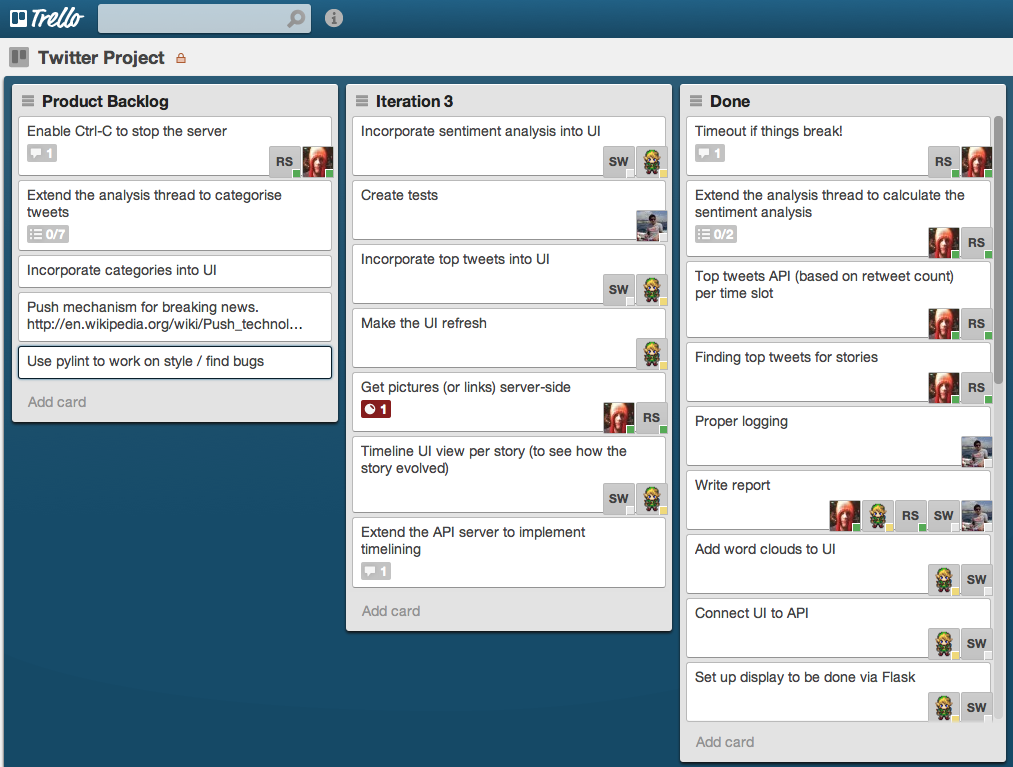
\includegraphics[scale=0.4]{trello1.png}
						\caption{Trello project management board}
			\end{figure}

		
		\subsection{Management policies}
		
		\subsection{Management of knowledge transfer within the group}
	
  

\end{document}
